\documentclass[12pt]{amsart}
\usepackage[utf8]{inputenc}
\usepackage[
backend=biber,
style=numeric,
maxbibnames=99,
sorting=ynt
]{biblatex}
\usepackage{amsmath,amssymb,amsthm}
\usepackage{tikz}
\usepackage{standalone}
\usepackage{svg}
\usepackage{gensymb}
\usepackage{float}
\usepackage{geometry}
\usepackage{hyperref}
\usepackage{graphicx, animate}
\usepackage{caption, subcaption}
\usepackage{pgffor}
\usepackage{mathtools}
\usepackage{array}
\addbibresource{bibliography.bib}
\usepackage{hyperref,thmtools}
\linespread{1.5}
 
% Override ugly default link
\hypersetup{
  colorlinks   = true, %Colours links instead of ugly boxes
  urlcolor     = blue, %Colour for external hyperlinks
  linkcolor    = blue, %Colour of internal links
  citecolor   = blue    %Colour of citations
}

\begin{document}

\begin{section}{Introduction}
    Temporal networks are networks whose nodes and edges change in time. In this thesis we look to model temporal networks. That is, describe the temporal network using mathematical language. 
    % Why temp nets are important
    The modelling of temporal networks is an important task in many real world applications including symptom interactions for mental health \cite{jordan2020current,contreras2020temporal}, epidemiology \cite{masuda2013predicting}, and protein interactions \cite{lucas2021inferring,jin2009identifying}.

    % Temp nets are dynam systs
    Temporal networks can be seen as a system in which points, in our case nodes in a network, whose states, the edges connecting them, that vary dependent in time, a dynamical system. 

    % Hard to find dynam systs because of discrete events 
    Discovering the underlying equations governing these dynamical systems proves challenging. That is because changes in network structure are typically observed in the form of discrete jumps from one state to another, for example an edge between two nodes not being observed at the first time step then being observed at the next.

    % We are proposing a solution
    In this thesis, we propose a hybrid statistical and deep learning framework. That is a framework in which a neural network is used to model probabilistic values of the temporal network. This framework allows us to model temporal networks as continuous-time dynamical systems, discover a fitting set of differential equations describing it, and, exploiting that discovery, predict the time evolution of a network.

    % DEs are useful for modelling interacting states
    Differential equations are useful for modelling systems where the state of one variable can effect the trajectories of other variables. 

    % Temp nets have interacting states 
    We observe this behavior in temporal networks; nodes' connections within the network can influence the observation of edges between other nodes, for example the phenomenon observed in \cite{newman2001clustering,capocci2006preferential}, where a node is more likely to gain the connections the more connections it has (preferential attachment). With this in mind we might wish to draw on the rich mathematical literature of differential equation modelling.

    % Temp net events are discrete
    In the common representation of networks as binary-valued adjacency matrices, matrices where the observation, or lack thereof, of an edge is represented as a 1 or 0 respectively, the events recorded in a temporal sequence of networks correspond to the appearance or the disappearance of link.
   
    % Difficult to model discrete events
    Because of the discrete nature of events, directly modelling the temporal networks as dynamical systems would require us to handle discrete jumps.
    The topological nature of temporal networks, and the discontinuous character of their temporal evolution, make it challenging to use differential equations techniques.

    % We propose a solution
    Here, we overcome the discreteness problem by interpreting networks as a well established statistical model for complex networks, that embeds nodes in a continuous, low-dimensional metric space by using a truncated singular value decomposition (Random Dot Product Graphs\cite{athreya2017statistical}). In this way we translate the hard problem of modelling discrete events in the space of networks to the easier problem of modelling continuous change in the embedding space. 
    
    % Our solution is interpretable because we use symb reg
    We then define and use systems of Neural Network Differential Equations (NNDE)\cite{SciML_C_Rak} to approximate the time evolution of the embedding space, and symbolic regression techniques to discover the functional form of the fitted NNDEs. These functional forms are interpretable (as they read as classic differential equations) and allow us to predict forward in time the evolution of the temporal networks.

    % We propose a solution
    In this manuscript, we show that the temporal network prediction problem can be successfully re-interpreted as a dynamical system modelling problem by taking the singular value decomposition of a sequence of adjacency matrices and training a NNDE to model an approximation to the underlying differential equation. We then go on to create a symbolic equation of this approximation. 

    % We will do some small tests on the proposed framework
    We apply our proposed framework to three small example temporal networks with the hope of exploring the limitations and strengths of the proposed framework. 

    % The framework can and should be tweaked to make it optimised
    The framework we are introducing is extremely flexible, and our research regarding the optimal structure of the Neural Networks used for the NNDEs is just started.
    We are confident that future research can identify more fitting Neural Network structures than the simple one adopted here.
    For this reason, we did not yet attempt to benchmark our model against other classic temporal network prediction methods.

    % The framework can be applied to lots of fields
    As it is completely general, we believe that the framework we are introducing can be usefully applied to areas of medicine, especially protein interaction networks; population dynamics for network ecology; and social network modelling. In particular, we discuss how specific domain knowledge relative to the prediction scenario can be taken into account, moving from NNDEs to Universal Differential Equations.
\end{section}

\begin{section}{Literature Review}

    \subsection{Temporal Networks}
        % Use of temp nets
        Temporal networks are used to describe a series of interactions across time.
        A temporal network $G$ is defined as:  
        \begin{align}
            G=\{ {_t} G=({_t} N, {_t} E)\} _{t \in 1\ldots T } 
        \end{align}
        $_t x \in {_t} N, {_t} e\in {_t} E$, where ${_t} x, {_t} e$ are nodes and edges at time $t$ respectively, and ${_t} N, {_t} E$ are the sets of nodes and edges at time $t$ respectively.
        An example of this can be found in \autoref{method nets}.
        
        %representations of temp nets as adj lists
        This can be represented in many ways, for example as a series of interactions. The series of interactions is generally represented as a list of tuples containing the node that interacted and the time that the interaction took place. 
        \begin{align}
            G=\{(i, j, t)|\space i,j\in {_t} N, (i\leftrightarrow j)\in {_t}E \}
        \end{align}
        
        % representation of temp nets as adj mats
        A temporal network can also be represented as a sequence of adjacency matrices. In the representation of a series of adjacency matrices, the columns and rows of the matrix each refer to each of the nodes. In this way, if an edge exists between nodes $i$ and $j$, the entry $(i,j)$ of the adjacency matrix will be 1; if an edge does not exist the entry will be 0.
        \begin{align}
            _t G &= {_t} A\\
            _t A_{ij} &=  
            \left\{
                \begin{array}{ll} 
                1 & (i\leftrightarrow j)\in {_t} E\\
                0 & otherwise
                \end{array}
            \right.
        \end{align}
        The row $_t A_{i\cdot}$ describes the outgoing edges of the node $i$, while the column $_t A_{\cdot j}$ describes the incoming edges of the node $j$.

        % Uses of temp nets
        Temporal networks are present in many areas of research interest, ranging from symptom interactions in mental health\cite{jordan2020current,contreras2020temporal}, to epidemiology\cite{masuda2013predicting}, protein interactions\cite{lucas2021inferring,jin2009identifying}, and social networks\cite{moinet2015burstiness,hanneke2010discrete}.     
        
        % Overview of modelling attempts
        Generally attempts to model temporal networks either model the change in node state or the change in network structure.
        
        The node state describes some information about that node:
        \begin{align}
            _t x &= (m_1,\ldots, m_p)
        \end{align}
        Where $m_i$ is some metadata about the node $_t x$.

        An example of modelling the change in a node state could be the severity of a symptom at a given time, as in \Citeauthor{contreras2020temporal}\cite{contreras2020temporal}. Where the node $_t x$ represents the symptom and $m_1$ would represent the severity of that symptom. 
        
        Other effort focus on modelling the changing structure of the network as in \Citeauthor{sanna2021link}\cite{sanna2021link}, which looks to model $_t G$ as a whole.

        % Intro contreras as attempt to model changes in nodes
        \Citeauthor{contreras2020temporal}\cite{contreras2020temporal} model the change in node state over time while the structure of the network remains constant. \Citeauthor{contreras2020temporal} look at the severity of symptoms over time, i.e. the state of the nodes, as a temporal network where the network structure remains constant. 
        
        % Contreras methods
        They use multilevel vector autoregression, a method that finds correlations between the current state of a variable and the states of variables at previous time steps \cite{singer2003applied}, to model how the current symptoms of people with paranoia might predict their future symptoms. These models were then used to create three networks that linked symptoms. 
        
        % Focal point of the paper is their temporal network
        Of particular interest to this thesis is the temporal network created by having a fully connected network of all symptoms including self-loops, where a symptom connects to itself; this self loop comes about from a symptom being correlated with itself from one time step to the next. The edge weights represent the extent to which the severity of each symptom at time $(t)$ predicts the severity of itself and other symptoms at time $(t+1)$. 
        
        % Why this is the focal point
        This framework keeps the overall structure of the network fixed throughout time and so is not particularly flexible, but is extremely human interpretable and can be used to extrapolate and predict into the future. 

        % intro to paper as attempt to model node state
        In \cite{KARIMI20133476}, the \Citeauthor{KARIMI20133476} look to model the change in node state while the network structure changes. 
        
        % How network is represented
        \Citeauthor{KARIMI20133476} represent their temporal network as a series of interactions (a list of tuples in the form $(i,j,t)$, where $i,j$ are the nodes interacting and $t$ is the time the at which the interaction occurred). 
        
        % what state the paper attempts to model
        The authors use a model to predict when a node will change from state 0 to state 1, in practice this could represent whether a user of a social network believes a rumour, or an ecological patch being colonised. 
        
        % Model limitation
        Notably, in their model the node never changes back; this is done to keep the model analytically tractable, but does limit its usefulness in some contexts. In this model an organism could not become locally extinct in an ecological patch for example. 
        
        % Methods to model node state
        To model the change in a nodes' state, the model uses a sliding time window and if the fraction of interactions with nodes of state 1 within that time window exceeds a given threshold, the node switches to state 1 as well. 

        % Limitation of model
        In this work I aim to present a model for predicting the state of a node in the future. Instead, \Citeauthor{KARIMI20133476} aim to present a tool for understanding the spread of ideas, viruses, etc. within a network.

        % Intro to pasino et al as modelling structure of temp net
        \Citeauthor{sanna2021link}\cite{sanna2021link} model the change in the structure of a temporal network. 
        
        % temp net representation
        In this case the \Citeauthor{sanna2021link} represent the temporal network as a series of adjacency matrices, each matrix representing an observation of the changing network. 
        
        % Methods for embedding
        The authors look to model the structure of edges by using a spectral embedding (SVD). A spectral embedding uses the eigenvectors of a network's adjacency matrix to find vectors that represent the nodes of the network. The spectral embedding transforms their temporal sequence into a sequence of observations of a latent space. 
        
        % What is a latent space
        A latent space is a continuous space in which similar nodes (nodes with many of the same neighbours) are positioned near each other. In this space nodes are represented as points in a continuous, low dimensional space. Another feature of this latent space, is that the dot product of any two points in the space gives us the probability that the nodes related to those points are connected. 
        
        % methods for time series
        With this series of embeddings, the authors employ a variety of time series techniques to predict the network structure at future time steps.

    \subsection{UDEs and NNDEs}
        % Justification for DEs being useful
        In some temporal networks the state of a node might influence the evolution of its neighbours. For example, in social networks we often observe the power law distribution of edges, where the more neighbours a node has, the more likely they are to gain more neighbours\cite{zhao2012multi,garg2009evolution}. We also see that the state of symptoms (occurrence, severity, and distress), can influence the states of other symptoms in patients undergoing chemotherapy \cite{papachristou2019network,kalantari2022network}, and for mental health disorders \cite{contreras2020temporal}. As well as in ecological networks where the interactions of species are often represented as a network, and the populations of one species may influence the population growth of another \cite{elton2001animal,volterra1927variazioni}; that is, the state (in this case the population) of a species (node), may influence the movement of another species.
        
        % DEs have lots of research
        With the observation that nodes in real world temporal networks may influence others, differential equations or difference equations seem appropriate for modelling the evolution of nodes as there is a rich body of literature exploring these methods use in modelling interacting variables. 
        
        % The data we have is discrete, which is a problem for DEs
        One of the issues that the differential equation method encounters is the prevalence of discrete jumps of edges forming and decaying. Because of this we may consider exploring the possibility of using difference equations.  
    
        % time is continuous so good to have our model be cont too
        We note that the progression of the network is generally continuous even if the events happen as discrete jumps. Because of this, we may wish to preserve the continuous temporal progression in our model.
        

        %This approach may overcome the problem of discrete observations, by defining a progression function that will only predict discrete formation or decay of edges\cite{hanneke2010discrete}. However, this imposes a significant limitation on the temporal granularity with which we can predict the state of the network. We would be limited to the granularity our data is collected at. This may be a problem if for example we had a series of weekly or monthly observations of networks we would not be able to predict interactions at each day. We can overcome both this limitation and the discrete jump limitation by using random dot product graphs. Interpolation may be possible in this case, but we would have no way of knowing if the interpolation had any basis in the real world.
        
        % passino has discrete data but uses a method to view it as cont
        Looking at the work of Passino et al.\cite{sanna2021link}, the authors use random dot produce graphs\cite{athreya2017statistical} to approximate a temporal network as a matrix of probabilities of an edge existing between two nodes. In contrast to edges, these probabilities can evolve continuously, and so we can use differential equations to generate probabilistic networks at any temporal resolution we require. That is, we will be able to model the changes in the probabilities of edges continuous and from this, generate a network at any time step.

        %  we can use the same method we can view data as dynam sys and use DEs
        Using the method in Passino et al.\cite{sanna2021link}, we can treat the sequence of embeddings as a dynamical system and then use differential equation modelling in a continuous space. That is, once we have found a latent space for each network. We know that each point in this space refers to a specific node in the network, and so, as the network changes, so too does the position of each of the points in the latent space. We then look to model this movement using differential equations. 
        
        % Can use a new NN structure to make this framework very general
        Our aim for this framework to be as general as possible and note that there may not yet be enough domain knowledge to perform traditional differential equation modelling to the desired accuracy. For example in network ecology models can be useful, but not perfect XXX cite XXX. Hence, we might wish to build on these models rather than trying to create something entirely new. This can be achieved by using this partial domain knowledge using it to create a universal differential equation (UDE) \cite{SciML_C_Rak}.

        \subsubsection{Theory}

            % Overview of why UDEs are useful
            Developed by \Citeauthor{SciML_C_Rak}\cite{SciML_C_Rak}, Universal Iifferential Equation (UDEs) are a novel neural network architecture that aims to take the best of both traditional neural differential equation modelling and of flexible machine learning approaches to modelling. 

            If we consider a comparison to an Ordinary Differential Equation (ODE), the ODE is written as:
            \begin{align}
                y(0) &= y_0 \\
                \frac{dy}{dt}(t)&=f(t,y(t))
            \end{align}
            
            The UDE will incorporate some component of $f(t,y(t))\approx \hat f(t,y(t))$, and will learn the difference with a Neural Network (NN) such that:
            \begin{align}
                \label{UDE}
                y(0) &= y_0 \\
                \frac{dy}{dt}(t)&=\hat f(t,y(t))+NN(t,y(t), \theta)
            \end{align}
            Where $\theta$ is a vector of the parameters of the NN.
            % Structure of UDE
            UDEs combine domain knowledge in the form of a differential equation, with a neural network. This hybrid machine learning model is then trained on the observed data.
            
            % Overview of why UDEs are useful
            Combining the two allows for most of the movement in the data to be captured by the differential equation, which contains the domain knowledge. In this way the neural network will only need to learn a theoretically simpler equation, given that a part of the system has already been captured. 
            
            % Why this structure is useful
            This then allows the neural network to be smaller, require fewer data, and be trained much faster than traditional neural network models. Given the flexibility of neural networks, the use of UDEs is natural when modelling a process that is not entirely understood\cite{kidger2022neural}.
            
            % Software used for coding
            There is an ecosystem of packages specifically designed for performing machine learning with UDEs. The ecosystem is called SciML or scientific machine learning\cite{SciML_C_Rak}. Largely, the SciML ecosystem has been optimised for flexibility and efficiency with respect to models available and training performance. Given there does not seem to be any other ecosystem with this feature, it seemed like 
            an obvious choice.
        
        \subsubsection{Applications}
            Whilst there has been much interest in implementing UDEs and neural ODEs, much of this work has been focussed on physics informed neural network and physics informed ordinary differential equations (PINNs and PINODEs) \cite{karniadakis2021physics,GAO2021110079,krishnapriyan2021characterizing,roehrl2020modeling}, and on improving modelling of fluids \cite{mahmoudabadbozchelou2021data,nguyen2022physics}. Alongside this, and given UDEs have gained popularity in the last few years, there have been a number of studies exploring their usefulness in modeling the effect of restrictions due to COVID-19 on the virus' spread \cite{Dandekar2020.04.03.20052084}. Although there has been a large amount of research into the usefulness of these types of models, to the best of this author's knowledge they have never been applied to the problem of predicting temporal networks. This seems to be a natural fit for UDEs and neural ODEs, given we may know relatively little about the processes that govern the evolution of temporal networks, and any information we do have can be incorporated into the model.

    \subsection{Symbolic Regression}
        % What is symbolic regression
        Symbolic regression is a type of analysis that looks to find a relationship between input variables that describe the output variables. For symbolic regression, we define a set of equations that may be used to find this relationship. The algorithm then generates combinations of these equations to find an expression that matches the output variables. Because we define the set of potential equations, the resulting expression is interpretable by humans, as opposed to a NN for example. 

        % Why is symbolic regression useful
        Having interpretable models that capture underlying relations is relevant to all fields of study, and so the applications of symbolic regression are incredibly varied. 

        % Where has symbolic regression been used 
        Various methods of symbolic regression have been use in manufacturing systems, chemical systems, and tumor research\cite{can2011comparison,keith2021combining,yoshihara2013inferring}. As well research into improvements is still on going.

        % How is this done
        This can be achieved in many ways and remains active area of research. One of the most popular algorithms is genetic programming\cite{schmidt2009distilling}. 
        
        % How genetic programming works
        Genetic programming involves constructing a search tree using a genetic algorithm to yield a potential equation, which may match the data as well as numerically calculated partial derivatives of each of the input variables. 
        
        % Why are the derivatives important
        Comparing with these derivatives is useful as it helps to ensure that the produced function equations have some grounding in the real world process that generated the data. The search tree is then pruned by comparing the partial derivatives of the candidate equation, with partial derivatives calculated from data. This process is then iterated many times to generate a suitable equation.

        % What symbolic regression aims to solve
        The problem that symbolic regression aims to solve is to generate interpretable and ``meaningful'' equations from observed data. 
        
        % Examples of use of genetic programming
        For example, both \Citeauthor{schmidt2009distilling,bongard2007automated} test their methods' capacity for obtaining a symbolic equation with physical simulation data, various pendula specifically. A ``meaningful'' equation in this case would be one that adheres to the laws of physics.

        % Expalaination of schmidt
        Examples of genetic programming include discovering equations governing the movement of simple harmonic and chaotic double pendula from data\cite{schmidt2009distilling}. In this paper the authors present an evolutionary algorithm to generate multiple candidate functions that approximate the partial derivatives of each variable that are calculated directly from the data. 
        
        % Intro to bongard
        Another approach to symbolic regression can be found in \cite{bongard2007automated}. This paper proposes a method to find a symbolic equation that approximates a learned numerical equation rather than directly from data. 
        
        % How does this process work
        The candidate equation is then tested against the numerical equation in such a way that the difference between the two predictions are maximised. The algorithm will generate new initial conditions to find behaviour exhibited by the numerical equation, for example a fixed point, that is not exhibited by the functional equation. When a difference is found, the functional equation is adjusted to also exhibit the behaviour of the numerical equation. 
        
        % Limitations of this process
        Especially when using a neural network model as the numerical equation, it seems these process may not be useful if the initial conditions are outside the scope of the training data.
        
        % Benefits of combining UDEs and symbolic regression
        In very recent work, Kidger\cite{kidger2022neural}, demonstrates that, with UDEs, two of the assumptions necessary for symbolic regression can be overcome. Those are the necessity for paired observations and derivatives, as well as the assumption that the function can be expressed as a shallow tree of symbolic operations. We are modelling a differential equation, and so will have access to the derivatives of our numerical model at any point, as neural networks are easily differentiable. 

        % Usefulness of symbolic regression for nnde
        In \Citeauthor{SciML_C_Rak}\cite{SciML_C_Rak}, the authors demonstrate that using symbolic regression, as opposed to just an NNDE, can improve the accuracy of extrapolating. One aspect of this improvement is having accurate numerical derivative to compare to. To ensure this, it is important that the data is sampled very frequently. This seems integral to the accuracy of the found equation. 
\end{section}

\begin{section}{Methodology}

        % Goal is to predict next time steps
        We are given a sequence of graphs, and our goal is to predict the next graph in the sequence. 
        
        % How we achieve this goal
        To achieve this, we reinterpret each graph as a sequence of points in a latent space; that is, a space in which similar vertices (ones with many of the same neighbours) are mapped to a similar point in space.
        We then Train a Neural Network Differential Equation (NNDE) to approximate the rate of change of the points in this latent space. With this numerical equation we can then use symbolic regression techniques to find a functional equation that matches the numerical equation. Using this process we discover an interpretable function that governs the evolution of a differential equation.

        \begin{figure}
            \centering
            \begin{subfigure}[c]{1\textwidth}
                \begin{tabular}{llll}
                \begin{subfigure}[c]{0.25\textwidth}
                    \centering
                    \resizebox{.6\width}{!}{\documentclass{standalone}
\usepackage{amsmath,amssymb,amsthm}
\usepackage{tikz}
\usetikzlibrary{decorations.markings}
\usetikzlibrary{arrows,automata}
\usetikzlibrary{positioning}
\usetikzlibrary{arrows.meta,positioning}

\begin{document}
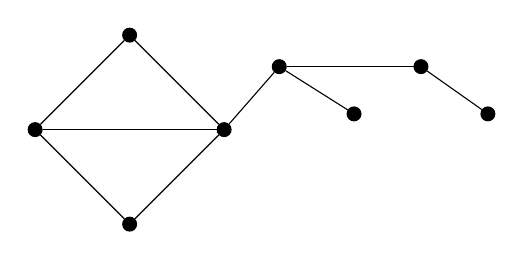
\begin{tikzpicture}[
    mycircle/.style={
        circle,
        draw=black,
        fill=black,
        fill opacity = 1,
        inner sep=0pt,
        minimum size=5pt,
        font=\small},
    nocircle/.style={
        circle,
        draw=black,
        fill=black,
        fill opacity = 1,
        inner sep=0pt,
        minimum size=0.45pt,
        font=\small},
    targetcircle/.style={
        circle,
        draw=red,
        fill=red,
        fill opacity = 1,
        inner sep=0pt,
        minimum size=5pt,
        font=\small},
    myarrow/.style={-},
    dottedarrow/.style={-,dashed},
    thiccarrow/.style={-,line width=0.9pt},
    node distance=1.2cm and 1.5cm
]

\begin{scope}
    \begin{scope}[rotate=90]
        \foreach \x/\y in {0/0,90/1,180/2, 270/3}{ % color in outer layer
        \node[mycircle] (\y) at (canvas polar cs: radius=1.2cm,angle=\x){};
        }
    \end{scope}

    \path[every node/.style={font=\sffamily\small}]
        % (0) edge [color=black] (1)
        (0) edge [color=black] (1)
        (0) edge [color=black] (3)
        (1) edge [color=black] (2)
        (1) edge [color=black] (3)
        (2) edge [color=black] (3);

    \node[mycircle] (a) at (1.9, 0.8) {};
    \node[mycircle] (b) at (2.85, 0.2) {};
    \node[mycircle] (c) at (3.7, 0.8) {};
    \node[mycircle] (d) at (4.55, 0.2) {};

    \path[every node/.style={font=\sffamily\small}]
        (3) edge [color=black] (a)
        (a) edge [color=black] (b)
        (a) edge [color=black] (c)
        (c) edge [color=black] (d);


\end{scope}
\end{tikzpicture}
\end{document}}
                    \label{method net, a}
                \end{subfigure}
                &
                \centering
                \begin{subfigure}[c]{0.25\textwidth}
                    \centering
                    \resizebox{.6\width}{!}{\documentclass{standalone}
\usepackage{amsmath,amssymb,amsthm}
\usepackage{tikz}
\usetikzlibrary{decorations.markings}
\usetikzlibrary{arrows,automata}
\usetikzlibrary{positioning}
\usetikzlibrary{arrows.meta,positioning}

\begin{document}
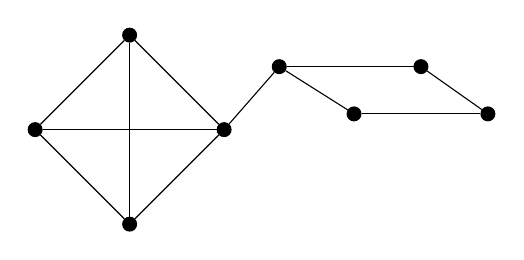
\begin{tikzpicture}[
    mycircle/.style={
        circle,
        draw=black,
        fill=black,
        fill opacity = 1,
        inner sep=0pt,
        minimum size=5pt,
        font=\small},
    nocircle/.style={
        circle,
        draw=black,
        fill=black,
        fill opacity = 1,
        inner sep=0pt,
        minimum size=0.45pt,
        font=\small},
    targetcircle/.style={
        circle,
        draw=red,
        fill=red,
        fill opacity = 1,
        inner sep=0pt,
        minimum size=5pt,
        font=\small},
    myarrow/.style={-},
    dottedarrow/.style={-,dashed},
    thiccarrow/.style={-,line width=0.9pt},
    node distance=1.2cm and 1.5cm
]

\begin{scope}
    \begin{scope}[rotate=90]
        \foreach \x/\y in {0/0,90/1,180/2, 270/3}{ % color in outer layer
        \node[mycircle] (\y) at (canvas polar cs: radius=1.2cm,angle=\x){};
        }
    \end{scope}

    \path[every node/.style={font=\sffamily\small}]
        % (0) edge [color=black] (1)
        (0) edge [color=black] (1)
        (0) edge [color=black] (2)
        (0) edge [color=black] (3)
        (1) edge [color=black] (2)
        (1) edge [color=black] (3)
        (2) edge [color=black] (3);

    \node[mycircle] (a) at (1.9, 0.8) {};
    \node[mycircle] (b) at (2.85, 0.2) {};
    \node[mycircle] (c) at (3.7, 0.8) {};
    \node[mycircle] (d) at (4.55, 0.2) {};

    \path[every node/.style={font=\sffamily\small}]
        (3) edge [color=black] (a)
        (a) edge [color=black] (b)
        (a) edge [color=black] (c)
        (c) edge [color=black] (d)
        (b) edge [color=black] (d);


\end{scope}
\end{tikzpicture}
\end{document}}
                    \label{method net, b}
                \end{subfigure}
                &
                $\cdots$
                &
                \centering
                \begin{subfigure}[c]{0.25\textwidth}
                    \centering
                    \resizebox{.6\width}{!}{\documentclass{standalone}
\usepackage{amsmath,amssymb,amsthm}
\usepackage{tikz}
\usetikzlibrary{decorations.markings}
\usetikzlibrary{arrows,automata}
\usetikzlibrary{positioning}
\usetikzlibrary{arrows.meta,positioning}

\begin{document}
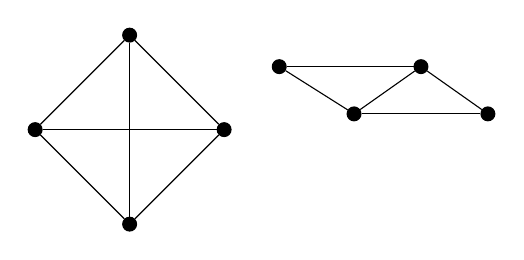
\begin{tikzpicture}[
    mycircle/.style={
        circle,
        draw=black,
        fill=black,
        fill opacity = 1,
        inner sep=0pt,
        minimum size=5pt,
        font=\small},
    nocircle/.style={
        circle,
        draw=black,
        fill=black,
        fill opacity = 1,
        inner sep=0pt,
        minimum size=0.45pt,
        font=\small},
    targetcircle/.style={
        circle,
        draw=red,
        fill=red,
        fill opacity = 1,
        inner sep=0pt,
        minimum size=5pt,
        font=\small},
    myarrow/.style={-},
    dottedarrow/.style={-,dashed},
    thiccarrow/.style={-,line width=0.9pt},
    node distance=1.2cm and 1.5cm
]

\begin{scope}
    \begin{scope}[rotate=90]
        \foreach \x/\y in {0/0,90/1,180/2, 270/3}{ % color in outer layer
        \node[mycircle] (\y) at (canvas polar cs: radius=1.2cm,angle=\x){};
        }
    \end{scope}

    \path[every node/.style={font=\sffamily\small}]
        % (0) edge [color=black] (1)
        (0) edge [color=black] (1)
        (0) edge [color=black] (2)
        (0) edge [color=black] (3)
        (1) edge [color=black] (2)
        (1) edge [color=black] (3)
        (2) edge [color=black] (3);

    \node[mycircle] (a) at (1.9, 0.8) {};
    \node[mycircle] (b) at (2.85, 0.2) {};
    \node[mycircle] (c) at (3.7, 0.8) {};
    \node[mycircle] (d) at (4.55, 0.2) {};

    \path[every node/.style={font=\sffamily\small}]
        (b) edge [color=black] (c)
        (a) edge [color=black] (b)
        (a) edge [color=black] (c)
        (c) edge [color=black] (d)
        (b) edge [color=black] (d);


\end{scope}
\end{tikzpicture}
\end{document}}
                    \label{method net, c}
                \end{subfigure}
                
                \end{tabular}
                \caption{Example sequence of networks.}
                \label{method nets}
                
            \end{subfigure}
            \begin{subfigure}[c]{1\textwidth}
                \begin{tabular}{llll}
                    $\begin{bmatrix}
                        \cdot & 1 & 1 & 1 & \cdot & \cdot & \cdot & \cdot\\
                        1 & \cdot & 1 & \cdot & \cdot & \cdot & \cdot & \cdot\\
                        1 & 1 & \cdot & 1 & 1 & \cdot & \cdot & \cdot\\
                        1 & \cdot & 1 & \cdot & \cdot & \cdot & \cdot & \cdot\\
                        \cdot & \cdot & 1 & \cdot & \cdot & 1 & 1 & \cdot\\
                        \cdot & \cdot & \cdot & \cdot & 1 & \cdot & \cdot & \cdot\\
                        \cdot & \cdot & \cdot & \cdot & 1 & \cdot & \cdot & 1\\
                        \cdot & \cdot & \cdot & \cdot & \cdot & \cdot & 1 & \cdot
                    \end{bmatrix}$
                    &
                    $\begin{bmatrix}
                        \cdot & 1 & 1 & 1 & \cdot & \cdot & \cdot & \cdot\\
                        1 & \cdot & 1 & 1 & \cdot & \cdot & \cdot & \cdot\\
                        1 & 1 & \cdot & 1 & 1 & \cdot & \cdot & \cdot\\
                        1 & 1 & 1 & \cdot & \cdot & \cdot & \cdot & \cdot\\
                        \cdot & \cdot & 1 & \cdot & \cdot & 1 & 1 & \cdot\\
                        \cdot & \cdot & \cdot & \cdot & 1 & \cdot & \cdot & 1\\
                        \cdot & \cdot & \cdot & \cdot & 1 & \cdot & \cdot & 1\\
                        \cdot & \cdot & \cdot & \cdot & \cdot & 1 & 1 & \cdot
                    \end{bmatrix}$
                    &
                    $\cdots$
                    &
                    $\begin{bmatrix}
                        \cdot & 1 & 1 & 1 & \cdot & \cdot & \cdot & \cdot\\
                        1 & \cdot & 1 & 1 & \cdot & \cdot & \cdot & \cdot\\
                        1 & 1 & \cdot & 1 & \cdot & \cdot & \cdot & \cdot\\
                        1 & 1 & 1 & \cdot & \cdot & \cdot & \cdot & \cdot\\
                        \cdot & \cdot & \cdot & \cdot & \cdot & 1 & 1 & \cdot\\
                        \cdot & \cdot & \cdot & \cdot & 1 & \cdot & 1 & 1\\
                        \cdot & \cdot & \cdot & \cdot & 1 & 1 & \cdot & 1\\
                        \cdot & \cdot & \cdot & \cdot & \cdot & 1 & 1 & \cdot
                    \end{bmatrix}$
                    
                \end{tabular}
                \caption{Sequence of sparse adjacency matrices associated with the networks in \autoref{method nets}.}
                \label{method adjacency}
            \end{subfigure}
    
            \begin{tabular}{llll}

            \end{tabular}
    
            \caption{Visual illustration of the proposed framework.}
            \label{framework illustration}
        \end{figure} 

    \subsection{Singular Value Decomposition and Random Dot Product Graphs}
            \label{svd}
            % Over view of section
            In this section we discuss the Singular Value Decomposition (SVD) of a matrix, and its usefulness in creating Random Dot Product Graphs (RDPG).

            % Definition of SVD
            We define the matrix $A$ to be a real $m \times n$ with $n \le m$. $A$ can be expressed as \cite{forsythe1967computer}:
            \begin{align}
                A&=l\sqrt{\Sigma} \sqrt{\Sigma} r' \\
                A&=L R'
            \end{align}
            Where $L, R$ are real valued, orthonormal matrices. The columns of $L$ consist of the $n$ largest eigenvectors of $AA'$ and the columns $R$ consist of the eigenvectors of $A'A$. $\Sigma$ is a diagonal matrix whose entries are the square root of the positive eigenvalues of $A'A$ in decreasing order.

            % How to reduce problem size
            In order to reduce the problem size, we can truncate the $L,R$ to the first $d$ columns to yield, $\hat L, \hat R$ such that:

            \begin{align}
                A &\approx \hat L \hat R' \\
                \hat A &= \hat L \hat R'
                \label{approx}
            \end{align}


            % Supposed to be how to interpret this as RDPG but is bad
            The approximation of $A$ is defined as $\hat A$ and is given by \autoref{approx} can be interpreted as a graph where the entry $(i,j)$ of the matrix is the probability that an edge $(i \leftrightarrow j)$ exists. This approximation of $A$ is an RDPG\cite{athreya2017statistical}.
     
            % Introduce problem of alignment
            It is important to note that the SVD is not unique. The distances between points will be the same for every embedding, but the orientation may be different, and so, if the SVD of each time step is not aligned, learning will be effectively impossible as we will essentially be trying to model random noise. 
            
            % How to solve alignment problem
            Here, we can use Procrustes alignment\cite{DotProductGraphs} to align the matrices after they have been generated.
            
            % SVD can give a latent space embedding
            The SVD can be considered to give a latent space representation of the matrix\cite{hoff2002latent}. That is, the rows of the matrices $\hat L,\hat R$ can be viewed as vector points in a $d$-dimensional space, where $d$ is the number of singular values we take for our SVD truncation. In this space similar nodes in the network are mapped to similar points in space. A visual representation of this process can be seen in \autoref{framework illustration}. 
            
            % Explicit process for how we process our data
            When obtaining the RDPGs for our temporal network, we take each network observation \autoref{method nets} and represent them in the form of an adjacency matrix \autoref{method adjacency}. We then use a truncated singular value decomposition to reduce the dimensionality of our adjacency matrices\cite{golub1971singular}. 
            
            % Introduce problem of loss from SVD
            This truncation introduces some loss, but can dramatically reduce the size of our problem. \Citeauthor{Runghen2021}\cite{Runghen2021} effectively employ this method to reduce a problem involving over 130,000 visitors to a 6 dimensional latent space, whilst preserving 70\% of the information.

            % What code we use
            To execute the SVD we use the ARPACK Julia package \cite{lehoucq1998arpack}. This package uses an iterative approach to approximate the eigenvectors and singular values of each of our adjacency matrices\cite{lehoucq1996deflation}.    

    \subsection{Neural Network Differential Equation}
        Once we have the SVD embedding of points, we look to model the trajectories of a target point. That is, with some input data, point location, distance to neighbours, etc, we want to model the differential equation that governs the movement of a point. 
        % Modelling multiple points
        Notably this method can be used to model multiple points by simply changing the node being predicted and trained on. 
            
        From \autoref{UDE} our problem can be represented as the UDE:
        \begin{align}
            \frac{d \hat A}{dt} &= \hat f(t,\hat A(t)) + NN(t, \hat A, \theta)
        \end{align}
        The focus of this thesis is to understand the behaviour of the neural network when modelling temporal neural networks. Hence, we set $\hat f(t, \hat A(t))=0 \space \forall t$. With this, the problem becomes:
        \begin{align}
            \frac{d \hat A}{dt} &= NN(t, \hat A, \theta)
        \end{align}
        A special case of a UDE called a Neural Network Differential Equation(NNDE).

        In this thesis, as a proof of concept, we focus on a modelling the change in structure of a single node, referred to as the target node $u$, where $u(t)={_t}\hat L_{1\cdot}$. To model $u$ we use the direction vectors from $u$ to its $k$ (15) nearest neighbours in $\hat L$. We define the function $K(\hat L(t), k)$ to find the direction vectors of the $k$ nearest neighbours to $u(t)$. We use the function $K$ to limit the complexity of our model.

        \begin{align}
            \frac{du}{dt} &= NN(t, K(\hat L, k), \theta)
        \end{align}

        Because we are only modelling the movement of a single node, we assume that we have access to the rest of the network structure at every time step for the prediction. This would likely not be the case in a real world application, but will allow us to observe some of the strengths and weaknesses of this framework in a controlled setting. If we wanted to predict the whole network we would extrapolate out every point and use the dot product of each point to predict the edges.
        
        Here we train a neural network to approximate the function $g(u(t),t)=NN(u(t),t,\theta)$. Where $\theta$ is the parameters of the neural network.

        
        To obtain a suitable set of parameters $\theta$, we make use of the SciML ecosystem of packages in the Julia programming language\cite{SciML_C_Rak}.    


    % Symbolic Regression Explaination
    
    \subsection{Symbolic Regression}
        With our trained NNDE, we have a black box that approximates the system that governs the movement of the target node in the embedded space. To make this more interpretable. We then look to approximate this black box into a combination of known functions using symbolic regression\cite{pysr}.
        
        We use the genetic programming algorithm found in \cite{pysr}. The process for which can be seen in \autoref{symbreg}.

        \begin{figure}
            \centering
            \resizebox{\width}{!}{\documentclass{standalone}
\usepackage{amsmath,amssymb,amsthm}
\usepackage{tikz}

\usetikzlibrary{decorations.markings}
\usetikzlibrary{arrows,automata}
\usetikzlibrary{positioning}
\usetikzlibrary{arrows.meta,positioning}

\begin{document}
\begin{tikzpicture}[
    mycircle/.style={
        circle,
        draw=black,
        fill=black,
        fill opacity = 1,
        inner sep=0pt,
        minimum size=5pt,
        font=\small},
    nocircle/.style={
        circle,
        draw=black,
        fill=black,
        fill opacity = 1,
        inner sep=0pt,
        minimum size=0.45pt,
        font=\small},
    targetcircle/.style={
        circle,
        draw=red,
        fill=red,
        fill opacity = 1,
        inner sep=0pt,
        minimum size=5pt,
        font=\small},
    myarrow/.style={->, -{Latex[length=3mm, width=2mm]}},
    dottedarrow/.style={-,dashed},
    thicccarrow/.style={->,line width=5pt},
    node distance=1.2cm and 1.5cm
]


\begin{scope}
    \begin{scope}
        \node[draw,text width=4cm] (a) at (0,0) {Randomly generate a set of candidate equations from a given set of operations};

        \node[draw,text width=4cm] (b) at (0,-4) {Simplifies and optimises any parameters in the candidate equations};

        \node[draw,text width=4cm] (c) at (5.5,-6.5) {Creates a tournament to test the fitness of each equation. The most fit equation is selected to go be re-randomised with a probability $p$, the next most fit is selected with probability $p(1-p)$};

        \node[draw,text width=4cm] (d) at (5.5,-0.5) {Re-randomises the selected equation to generate a new set of candidate equations};

        \node[draw,text width=4cm] (e) at (0,-9) {The fittest equation at each complexity is stored and returned};
    \end{scope}


    \path[every node/.style={font=\sffamily\small}] 
        (a) edge[myarrow] [color=black] (b)
        (b) edge[myarrow] [color=black] (c)
        (d) edge[myarrow] [color=black] (b)
        (c) edge[myarrow] [color=black] (d)
        (b) edge[myarrow] [color=black] (e);
\end{scope}
\end{tikzpicture}
\end{document}}
            \caption{Illustration of the genetic programming symbolic regression process.}
            \label{symbreg}
        \end{figure}
        
        The fitness of a candidate function is determined by comparing the predicted value to the given data, as well as the derivatives of the candidate equations to numerically found partial derivatives of the data variable.

        For this process we need to define a set of functions which the algorithm will use to generate a tree of functions to find the best approximation to our NNDE with. When using this method we are usually required to make two assumptions: that we have paired observations of $u(t), \frac{du}{dt}$, and that the tree of expressions we will need is shallow. We will train the symbolic regression on the predictions of the neural network. By doing this, we can remove these assumptions\cite{kidger2022neural}.

    \subsection{Reconstructing the Temporal Network}
        To recover a final prediction of the edges of $u$, we multiply the point vector of $u$ with the matrix $R'$. This gives a vector of probabilities of connections between the target node and the rest of the network. As the results can be interpreted as a probability, the most likely graph is given by setting any entry with a value of $0.5$ or higher to one (predict that the edge exists), and setting any entry with a value of less than $0.5$ to zero (predict that an edge does not exist).
\end{section}

\begin{section}{Data}
    In this paper we simulate three temporal sequences of undirected graphs. For each sequence we will be modelling the node in red, we will refer to this as the target node. For each sequence we train the model on the first 25 time steps and compare the predictions for the next 15 time steps. For clarity, each diagram \autoref{2community train series} \autoref{longTail train series} \autoref{3community train series} has been simplified and illustrates the movement of the target node in each sequence.

    \subsection{Two Community System}
        The 2 community network has communities of size 40 and 50, each of which are fully connected. The target node is initially fully connected to the 50 node community. In our simplified diagram \autoref{2community train series, a} the 50 node community is represented by the 5 fully connected nodes, while the 40 node community is represented by the 4 node component. At each time step one edge is removed between the target node and the larger community and replaced with an edge between the target node and the smaller community \autoref{2community train series, b}. This process is then continued \autoref{2community train series, c} for thirty-five time steps to generate our training and test data. Once we have this data in the form of a sequence of adjacency matrices, we find the singular value decomposition using the framework described in \autoref{svd}.

        Figures obtained from \cite{Emma2023}.
        \begin{figure}[H]
            \centering
            \centering
            \begin{subfigure}[c]{0.3\textwidth}
                \centering
                \resizebox{.6\width}{!}{\documentclass{standalone}
\usepackage{amsmath,amssymb,amsthm}
\usepackage{tikz}
\usetikzlibrary{decorations.markings}
\usetikzlibrary{arrows,automata}
\usetikzlibrary{positioning}
\usetikzlibrary{arrows.meta,positioning}

\begin{document}
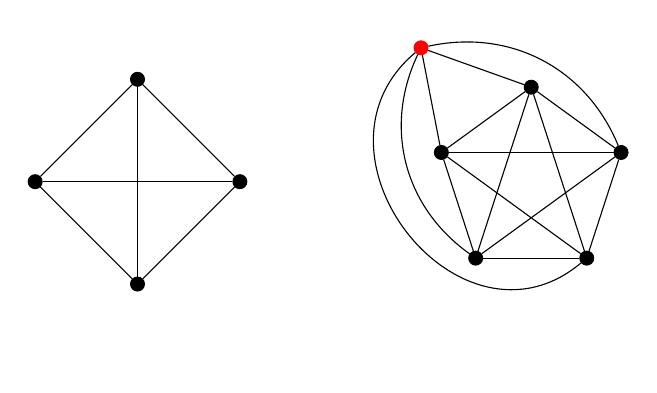
\begin{tikzpicture}[
    mycircle/.style={
        circle,
        draw=black,
        fill=black,
        fill opacity = 1,
        inner sep=0pt,
        minimum size=5pt,
        font=\small},
    nocircle/.style={
        circle,
        draw=black,
        fill=black,
        fill opacity = 1,
        inner sep=0pt,
        minimum size=0.45pt,
        font=\small},
    targetcircle/.style={
        circle,
        draw=red,
        fill=red,
        fill opacity = 1,
        inner sep=0pt,
        minimum size=5pt,
        font=\small},
    myarrow/.style={-},
    dottedarrow/.style={-,dashed},
    thiccarrow/.style={-,line width=0.9pt},
    node distance=1.2cm and 1.5cm
]


\begin{scope}
    \begin{scope}[rotate=90]
        \foreach \x/\y in {0/a,90/b,180/c, 270/d}{ % color in outer layer
        \node[mycircle] (\y) at (canvas polar cs: radius=1.3cm,angle=\x){};
        }
    \end{scope}

    \path[every node/.style={font=\sffamily\small}]
        (a) edge [color=black] (b)
        (a) edge [color=black] (c)
        (a) edge [color=black] (d)
        (b) edge [color=black] (c)
        (b) edge [color=black] (d)
        (c) edge [color=black] (d);
\end{scope}

\begin{scope}[xshift=5cm]
    \begin{scope}[rotate=90]
        \foreach \x/\y in {0/0,72/1,144/2, 216/3, 288/4}{ % color in outer layer
        \node[mycircle] (\y) at (canvas polar cs: radius=1.2cm,angle=\x){};
        }
    \end{scope}

    \path[every node/.style={font=\sffamily\small}]
        (0) edge [color=black] (1)
        (0) edge [color=black] (2)
        (0) edge [color=black] (3)
        (0) edge [color=black] (4)
        (1) edge [color=black] (2)
        (1) edge [color=black] (3)
        (1) edge [color=black] (4)
        (2) edge [color=black] (3)
        (2) edge [color=black] (4)
        (3) edge [color=black] (4);

    \node[targetcircle] (x) at (-1.4, 1.7) {};

    \path[every node/.style={font=\sffamily\small}]
        (x) edge [color=black] (0)
        (x) edge [color=black] (1)
        (x) edge [color=black, bend right=40] (2)
        (x) edge [color=black, out=220, in=-140, looseness=1.5] (3)
        (x) edge [color=black, bend left=40] (4);
\end{scope}
\end{tikzpicture}
\end{document}}
                \caption{$t=1$}
                \label{2community train series, a}
            \end{subfigure}
            \hfill
            \centering
            \begin{subfigure}[c]{0.3\textwidth}
                \centering
                \resizebox{.6\width}{!}{\documentclass{standalone}
\usepackage{amsmath,amssymb,amsthm}
\usepackage{tikz}
\usetikzlibrary{decorations.markings}
\usetikzlibrary{arrows,automata}
\usetikzlibrary{positioning}
\usetikzlibrary{arrows.meta,positioning}

\begin{document}
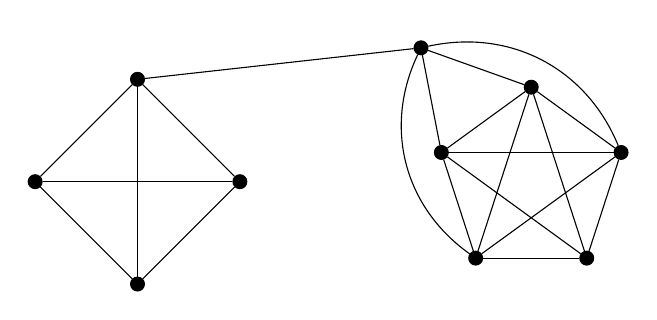
\begin{tikzpicture}[
    mycircle/.style={
        circle,
        draw=black,
        fill=black,
        fill opacity = 1,
        inner sep=0pt,
        minimum size=5pt,
        font=\small},
    nocircle/.style={
        circle,
        draw=black,
        fill=black,
        fill opacity = 1,
        inner sep=0pt,
        minimum size=0.45pt,
        font=\small},
    myarrow/.style={-},
    dottedarrow/.style={-,dashed},
    thiccarrow/.style={-,line width=0.9pt},
    node distance=1.2cm and 1.5cm
]
\begin{scope}
    \begin{scope}[rotate=90]
        \foreach \x/\y in {0/a,90/b,180/c, 270/d}{ % color in outer layer
        \node[mycircle] (\y) at (canvas polar cs: radius=1.3cm,angle=\x){};
        }
    \end{scope}

    \path[every node/.style={font=\sffamily\small}]
        (a) edge [color=black] (b)
        (a) edge [color=black] (c)
        (a) edge [color=black] (d)
        (b) edge [color=black] (c)
        (b) edge [color=black] (d)
        (c) edge [color=black] (d);
\end{scope}

\begin{scope}[xshift=5cm]
    \begin{scope}[rotate=90]
        \foreach \x/\y in {0/0,72/1,144/2, 216/3, 288/4}{ % color in outer layer
        \node[mycircle] (\y) at (canvas polar cs: radius=1.2cm,angle=\x){};
        }
    \end{scope}

    \path[every node/.style={font=\sffamily\small}]
        (0) edge [color=black] (1)
        (0) edge [color=black] (2)
        (0) edge [color=black] (3)
        (0) edge [color=black] (4)
        (1) edge [color=black] (2)
        (1) edge [color=black] (3)
        (1) edge [color=black] (4)
        (2) edge [color=black] (3)
        (2) edge [color=black] (4)
        (3) edge [color=black] (4);

    \node[mycircle] (x) at (-1.4, 1.7) {};

    \path[every node/.style={font=\sffamily\small}]
        (x) edge [color=black] (0)
        (x) edge [color=black] (1)
        (x) edge [color=black, bend right=40] (2)
        (x) edge [color=black, bend left=40] (4)
        (x) edge [color=black] (a);
\end{scope}
\end{tikzpicture}
\end{document}}
                \caption{$t=2$}
                \label{2community train series, b}
            \end{subfigure}
            \hfill
            \centering
            \begin{subfigure}[c]{0.3\textwidth}
                \centering
                \resizebox{.6\width}{!}{\documentclass{standalone}
\usepackage{amsmath,amssymb,amsthm}
\usepackage{tikz}
\usetikzlibrary{decorations.markings}
\usetikzlibrary{arrows,automata}
\usetikzlibrary{positioning}
\usetikzlibrary{arrows.meta,positioning}

\begin{document}
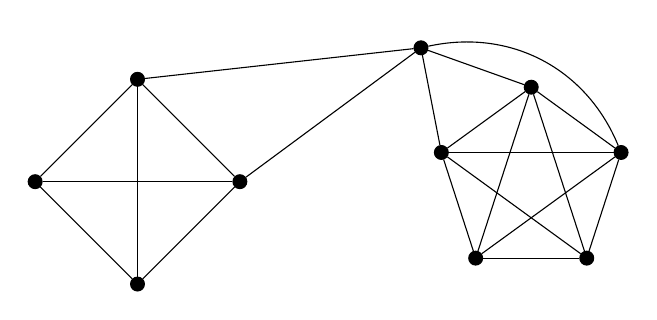
\begin{tikzpicture}[
    mycircle/.style={
        circle,
        draw=black,
        fill=black,
        fill opacity = 1,
        inner sep=0pt,
        minimum size=5pt,
        font=\small},
    nocircle/.style={
        circle,
        draw=black,
        fill=black,
        fill opacity = 1,
        inner sep=0pt,
        minimum size=0.45pt,
        font=\small},
    myarrow/.style={-},
    dottedarrow/.style={-,dashed},
    thiccarrow/.style={-,line width=0.9pt},
    node distance=1.2cm and 1.5cm
]
\begin{scope}
    \begin{scope}[rotate=90]
        \foreach \x/\y in {0/a,90/b,180/c, 270/d}{ % color in outer layer
        \node[mycircle] (\y) at (canvas polar cs: radius=1.3cm,angle=\x){};
        }
    \end{scope}

    \path[every node/.style={font=\sffamily\small}]
        (a) edge [color=black] (b)
        (a) edge [color=black] (c)
        (a) edge [color=black] (d)
        (b) edge [color=black] (c)
        (b) edge [color=black] (d)
        (c) edge [color=black] (d);
\end{scope}

\begin{scope}[xshift=5cm]
    \begin{scope}[rotate=90]
        \foreach \x/\y in {0/0,72/1,144/2, 216/3, 288/4}{ % color in outer layer
        \node[mycircle] (\y) at (canvas polar cs: radius=1.2cm,angle=\x){};
        }
    \end{scope}

    \path[every node/.style={font=\sffamily\small}]
        (0) edge [color=black] (1)
        (0) edge [color=black] (2)
        (0) edge [color=black] (3)
        (0) edge [color=black] (4)
        (1) edge [color=black] (2)
        (1) edge [color=black] (3)
        (1) edge [color=black] (4)
        (2) edge [color=black] (3)
        (2) edge [color=black] (4)
        (3) edge [color=black] (4);

    \node[mycircle] (x) at (-1.4, 1.7) {};

    \path[every node/.style={font=\sffamily\small}]
        (x) edge [color=black] (0)
        (x) edge [color=black] (1)
        (x) edge [color=black, bend left=40] (4)
        (x) edge [color=black] (a)
        (x) edge [color=black] (d);
\end{scope}
\end{tikzpicture}
\end{document}}
                \caption{$t=3$}
                \label{2community train series, c}
            \end{subfigure}
            \caption{First 3 time steps of the simplified, synthetic 2 community network. The red node represents the target node that we are aiming to model. The 4 node and 5 node fully connected components represent the 40 and 50 node communities of the sequence respectively. At each time step, an edge from the target node to the larger community is replaced with and edge from the target node to the smaller community.}
            \label{2community train series}
        \end{figure}
        The 2 community temporal network was selected to test whether this framework can be used to model a node changing communities in systems where there are no other processes occurring. Notably, the movement in the two community system is difficult for the neural network to learn because opposite sets of inputs need to result in the same output. In a simplified version of this system with only the nearest node as input, the input for the model begins as the position of the larger community at roughly $(0,-1)$ \autoref{2community series 1}. This input needs to move the target towards the top left. However, as the sequence progresses, the nearest neighbours will be the small community at roughly $(-1,0)$, which also needs to move the target node towards the top left. 

    \subsection{Long Tail System}
        In the long tail network \autoref{longTail train series}, we have a long chain with 50 nodes and a fully connected component with forty nodes at one end of the chain. This is used to orient the embedding and model. The SVD does not take into account the index of the individual node in the adjacency matrix; it only distinguishes based on their distance to each other. Because of this a chain of nodes, even when aligned, could be flipped when it is embedded. That is, between one time step and the next the first node in the chain could be aligned with the last node. With a large, connected group at one end however, that group will always be aligned with itself and so the rest of the chain will also be aligned properly. The target node starts attached to the node that is attached to this large component \autoref{longTail train series, a}. At each time step the target node move one node further down the tail \autoref{longTail train series, b}. Again, this is repeated to generate the training and test data \autoref{longTail train series, c}.
        \begin{figure}[H]
            \centering
            \begin{subfigure}[c]{0.3\textwidth}
                \centering
                \resizebox{.6\width}{!}{\documentclass{standalone}
\usepackage{amsmath,amssymb,amsthm}
\usepackage{tikz}
\usetikzlibrary{decorations.markings}
\usetikzlibrary{arrows,automata}
\usetikzlibrary{positioning}
\usetikzlibrary{arrows.meta,positioning}

\begin{document}
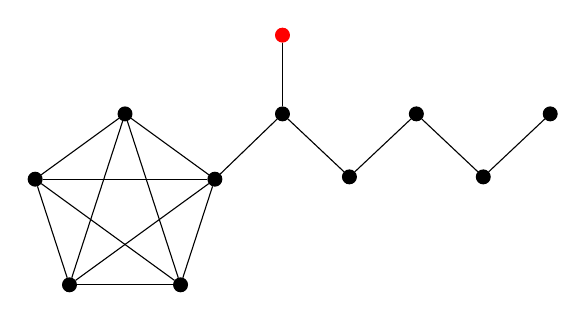
\begin{tikzpicture}[
    mycircle/.style={
        circle,
        draw=black,
        fill=black,
        fill opacity = 1,
        inner sep=0pt,
        minimum size=5pt,
        font=\small},
    nocircle/.style={
        circle,
        draw=black,
        fill=black,
        fill opacity = 1,
        inner sep=0pt,
        minimum size=0.45pt,
        font=\small},
    targetcircle/.style={
        circle,
        draw=red,
        fill=red,
        fill opacity = 1,
        inner sep=0pt,
        minimum size=5pt,
        font=\small},
    myarrow/.style={-},
    dottedarrow/.style={-,dashed},
    thiccarrow/.style={-,line width=0.9pt},
    node distance=1.2cm and 1.5cm
]
\begin{scope}
    \begin{scope}[rotate=90]
        \foreach \x/\y in {0/0,72/1,144/2, 216/3, 288/4}{ % color in outer layer
        \node[mycircle] (\y) at (canvas polar cs: radius=1.2cm,angle=\x){};
        }
    \end{scope}

    \path[every node/.style={font=\sffamily\small}]
        (0) edge [color=black] (1)
        (0) edge [color=black] (2)
        (0) edge [color=black] (3)
        (0) edge [color=black] (4)
        (1) edge [color=black] (2)
        (1) edge [color=black] (3)
        (1) edge [color=black] (4)
        (2) edge [color=black] (3)
        (2) edge [color=black] (4)
        (3) edge [color=black] (4);

    \node[mycircle] (a) at (2, 1.2) {};
    \node[mycircle] (b) at (2.85, 0.4) {};
    \node[mycircle] (c) at (3.7, 1.2) {};
    \node[mycircle] (d) at (4.55, 0.4) {};
    \node[mycircle] (e) at (5.4, 1.2) {};

    \path[every node/.style={font=\sffamily\small}]
        (4) edge [color=black] (a)
        (a) edge [color=black] (b)
        (b) edge [color=black] (c)
        (c) edge [color=black] (d)
        (d) edge [color=black] (e);

    \node[targetcircle] (x) at (2, 2.2) {};

    \path[every node/.style={font=\sffamily\small}]
        (x) edge [color=black] (a);
\end{scope}
\end{tikzpicture}
\end{document}}
                \caption{$t=1$}
                \label{longTail train series, a}
            \end{subfigure}
            \hfill
            \centering
            \begin{subfigure}[c]{0.3\textwidth}
                \centering
                \resizebox{.6\width}{!}{\documentclass{standalone}
\usepackage{amsmath,amssymb,amsthm}
\usepackage{tikz}
\usetikzlibrary{decorations.markings}
\usetikzlibrary{arrows,automata}
\usetikzlibrary{positioning}
\usetikzlibrary{arrows.meta,positioning}

\begin{document}
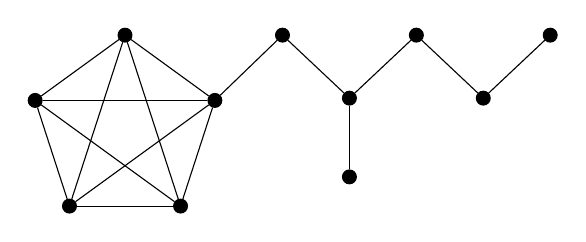
\begin{tikzpicture}[
    mycircle/.style={
        circle,
        draw=black,
        fill=black,
        fill opacity = 1,
        inner sep=0pt,
        minimum size=5pt,
        font=\small},
    nocircle/.style={
        circle,
        draw=black,
        fill=black,
        fill opacity = 1,
        inner sep=0pt,
        minimum size=0.45pt,
        font=\small},
    myarrow/.style={-},
    dottedarrow/.style={-,dashed},
    thiccarrow/.style={-,line width=0.9pt},
    node distance=1.2cm and 1.5cm
]

\begin{scope}
    \begin{scope}[rotate=90]
        \foreach \x/\y in {0/0,72/1,144/2, 216/3, 288/4}{ % color in outer layer
        \node[mycircle] (\y) at (canvas polar cs: radius=1.2cm,angle=\x){};
        }
    \end{scope}

    \path[every node/.style={font=\sffamily\small}]
        (0) edge [color=black] (1)
        (0) edge [color=black] (2)
        (0) edge [color=black] (3)
        (0) edge [color=black] (4)
        (1) edge [color=black] (2)
        (1) edge [color=black] (3)
        (1) edge [color=black] (4)
        (2) edge [color=black] (3)
        (2) edge [color=black] (4)
        (3) edge [color=black] (4);

    \node[mycircle] (a) at (2, 1.2) {};
    \node[mycircle] (b) at (2.85, 0.4) {};
    \node[mycircle] (c) at (3.7, 1.2) {};
    \node[mycircle] (d) at (4.55, 0.4) {};
    \node[mycircle] (e) at (5.4, 1.2) {};

    \path[every node/.style={font=\sffamily\small}]
        (4) edge [color=black] (a)
        (a) edge [color=black] (b)
        (b) edge [color=black] (c)
        (c) edge [color=black] (d)
        (d) edge [color=black] (e);

    \node[mycircle] (x) at (2.85, -0.6) {};

    \path[every node/.style={font=\sffamily\small}]
        (x) edge [color=black] (b);
\end{scope}
\end{tikzpicture}
\end{document}}
                \caption{$t=2$}
                \label{longTail train series, b}
            \end{subfigure}
            \hfill
            \centering
            \begin{subfigure}[c]{0.3\textwidth}
                \centering
                \resizebox{.6\width}{!}{\documentclass{standalone}
\usepackage{amsmath,amssymb,amsthm}
\usepackage{tikz}
\usetikzlibrary{decorations.markings}
\usetikzlibrary{arrows,automata}
\usetikzlibrary{positioning}
\usetikzlibrary{arrows.meta,positioning}

\begin{document}
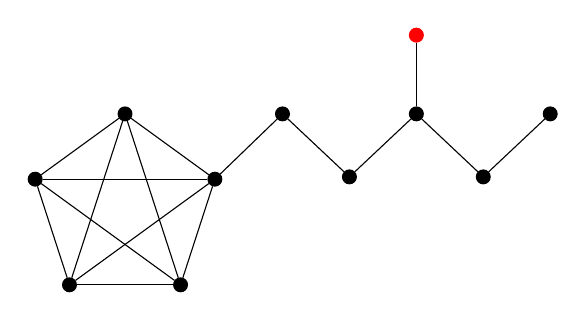
\begin{tikzpicture}[
    mycircle/.style={
        circle,
        draw=black,
        fill=black,
        fill opacity = 1,
        inner sep=0pt,
        minimum size=5pt,
        font=\small},
    nocircle/.style={
        circle,
        draw=black,
        fill=black,
        fill opacity = 1,
        inner sep=0pt,
        minimum size=0.45pt,
        font=\small},
    targetcircle/.style={
        circle,
        draw=red,
        fill=red,
        fill opacity = 1,
        inner sep=0pt,
        minimum size=5pt,
        font=\small},
    myarrow/.style={-},
    dottedarrow/.style={-,dashed},
    thiccarrow/.style={-,line width=0.9pt},
    node distance=1.2cm and 1.5cm
]

\begin{scope}
    \begin{scope}[rotate=90]
        \foreach \x/\y in {0/0,72/1,144/2, 216/3, 288/4}{ % color in outer layer
        \node[mycircle] (\y) at (canvas polar cs: radius=1.2cm,angle=\x){};
        }
    \end{scope}

    \path[every node/.style={font=\sffamily\small}]
        (0) edge [color=black] (1)
        (0) edge [color=black] (2)
        (0) edge [color=black] (3)
        (0) edge [color=black] (4)
        (1) edge [color=black] (2)
        (1) edge [color=black] (3)
        (1) edge [color=black] (4)
        (2) edge [color=black] (3)
        (2) edge [color=black] (4)
        (3) edge [color=black] (4);

    \node[mycircle] (a) at (2, 1.2) {};
    \node[mycircle] (b) at (2.85, 0.4) {};
    \node[mycircle] (c) at (3.7, 1.2) {};
    \node[mycircle] (d) at (4.55, 0.4) {};
    \node[mycircle] (e) at (5.4, 1.2) {};

    \path[every node/.style={font=\sffamily\small}]
        (4) edge [color=black] (a)
        (a) edge [color=black] (b)
        (b) edge [color=black] (c)
        (c) edge [color=black] (d)
        (d) edge [color=black] (e);

    \node[targetcircle] (x) at (3.7, 2.2) {};

    \path[every node/.style={font=\sffamily\small}]
        (x) edge [color=black] (c);
\end{scope}
\end{tikzpicture}
\end{document}}
                \caption{$t=3$}
                \label{longTail train series, c}
            \end{subfigure}\\
            \caption{First 3 time steps of the simplified, synthetic long tail network. The red node represents the target node that we are aiming to model. The fully connected, 5 node component represents a 50 node community at the end of the long tail. At each time step the target node moves one step further along the chain, away from the large community.}
            \label{longTail train series}
        \end{figure}    

        The long tail network was selected because the SVD performs poorly on highly diagonal matrices; that is matrices with long chains.  The long tail problem is difficult for the embedding because a large portion of the network is along the off diagonals; meaning that, to get an accurate embedding, the dimension of the embedding would need to be close to the length of the tail. As such we wish to see how the framework performs when it is presented with a system that the SVD cannot capture.

    \subsection{Three community System}
    We also simulate a sequence with three communities. The communities have sizes 40, 35, 30 and have 25, 24, and 23 edges to the target node respectively. In \autoref{3community train series} the communities have been simplified to have sizes of 5, 4, and 3. The target node starts connected to all of these communities with each community having a different number of edges \autoref{3community train series, a}. The community with the fewest edges between the target node will have one edge removed at each time step \autoref{3community train series, b}, and this process is repeated to create the required number of time steps \autoref{3community train series, c}.  
    \begin{figure}[H]
        \centering
        \centering
        \begin{subfigure}[c]{0.3\textwidth}
            \centering
            \resizebox{.6\width}{!}{\documentclass{standalone}
\usepackage{amsmath,amssymb,amsthm}
\usepackage{tikz}
\usetikzlibrary{decorations.markings}
\usetikzlibrary{arrows,automata}
\usetikzlibrary{positioning}
\usetikzlibrary{arrows.meta,positioning}

\begin{document}
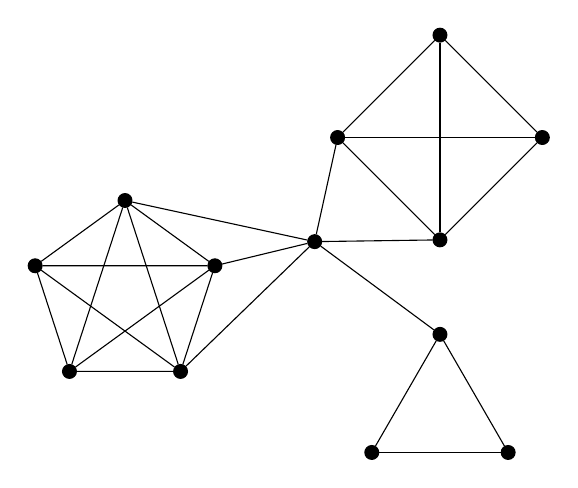
\begin{tikzpicture}[
    mycircle/.style={
        circle,
        draw=black,
        fill=black,
        fill opacity = 1,
        inner sep=0pt,
        minimum size=5pt,
        font=\small},
    nocircle/.style={
        circle,
        draw=black,
        fill=black,
        fill opacity = 1,
        inner sep=0pt,
        minimum size=0.45pt,
        font=\small},
    myarrow/.style={-},
    dottedarrow/.style={-,dashed},
    thiccarrow/.style={-,line width=0.9pt},
    node distance=1.2cm and 1.5cm
]
\begin{scope}
    \begin{scope}[rotate=-90]
        \foreach \x/\y in {0/a,90/b,180/c, 270/d}{ % color in outer layer
        \node[mycircle] (\y) at (canvas polar cs: radius=1.3cm,angle=\x){};
        }
    \end{scope}

    \path[every node/.style={font=\sffamily\small}]
        (a) edge [color=black] (b)
        (a) edge [color=black] (c)
        (a) edge [color=black] (d)
        (b) edge [color=black] (c)
        (b) edge [color=black] (d)
        (c) edge [color=black] (d);
\end{scope}

\begin{scope}[xshift=-4cm, yshift=-2cm, rotate=-72]
    \begin{scope}[rotate=90]
        \foreach \x/\y in {0/0,72/1,144/2, 216/3, 288/4}{ % color in outer layer
        \node[mycircle] (\y) at (canvas polar cs: radius=1.2cm,angle=\x){};
        }
    \end{scope}

    \path[every node/.style={font=\sffamily\small}]
        (0) edge [color=black] (1)
        (0) edge [color=black] (2)
        (0) edge [color=black] (3)
        (0) edge [color=black] (4)
        (1) edge [color=black] (2)
        (1) edge [color=black] (3)
        (1) edge [color=black] (4)
        (2) edge [color=black] (3)
        (2) edge [color=black] (4)
        (3) edge [color=black] (4);

    \node[mycircle] (x) at (0.1, 2.5) {};

    \path[every node/.style={font=\sffamily\small}]
        (x) edge [color=black] (0)
        (x) edge [color=black] (1)
        (x) edge [color=black] (4)
        (x) edge [color=black] (a)
        (x) edge [color=black] (d);
\end{scope}

\begin{scope}[yshift=-3.5cm, xshift=0cm]
    \begin{scope}[rotate=90]
        \foreach \x/\y in {0/0,120/1,240/2}{ % color in outer layer
        \node[mycircle] (\y) at (canvas polar cs: radius=1cm,angle=\x){};
        }
    \end{scope}

    \path[every node/.style={font=\sffamily\small}]
        (0) edge [color=black] (1)
        (0) edge [color=black] (2)
        (1) edge [color=black] (2)
        (x) edge [color=black] (0);
\end{scope}
\end{tikzpicture}
\end{document}}
            \caption{$t=1$}
            \label{3community train series, a}
        \end{subfigure}
        \hfill
        \centering
        \begin{subfigure}[c]{0.3\textwidth}
            \centering
            \resizebox{.6\width}{!}{\documentclass{standalone}
\usepackage{amsmath,amssymb,amsthm}
\usepackage{tikz}
\usetikzlibrary{decorations.markings}
\usetikzlibrary{arrows,automata}
\usetikzlibrary{positioning}
\usetikzlibrary{arrows.meta,positioning}

\begin{document}
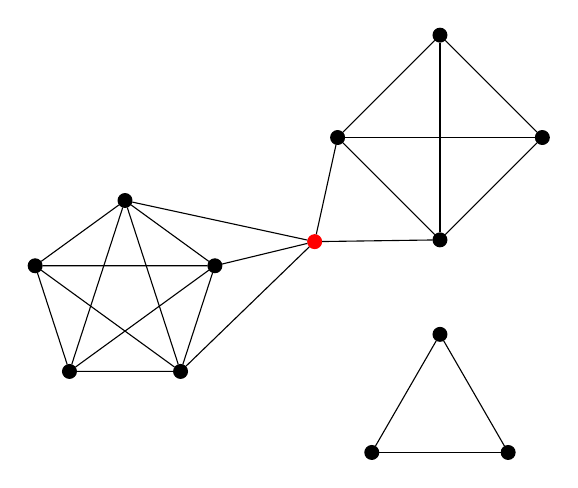
\begin{tikzpicture}[
    mycircle/.style={
        circle,
        draw=black,
        fill=black,
        fill opacity = 1,
        inner sep=0pt,
        minimum size=5pt,
        font=\small},
    nocircle/.style={
        circle,
        draw=black,
        fill=black,
        fill opacity = 1,
        inner sep=0pt,
        minimum size=0.45pt,
        font=\small},
    targetcircle/.style={
        circle,
        draw=red,
        fill=red,
        fill opacity = 1,
        inner sep=0pt,
        minimum size=5pt,
        font=\small},
    myarrow/.style={-},
    dottedarrow/.style={-,dashed},
    thiccarrow/.style={-,line width=0.9pt},
    node distance=1.2cm and 1.5cm
]
\begin{scope}
    \begin{scope}[rotate=-90]
        \foreach \x/\y in {0/a,90/b,180/c, 270/d}{ % color in outer layer
        \node[mycircle] (\y) at (canvas polar cs: radius=1.3cm,angle=\x){};
        }
    \end{scope}

    \path[every node/.style={font=\sffamily\small}]
        (a) edge [color=black] (b)
        (a) edge [color=black] (c)
        (a) edge [color=black] (d)
        (b) edge [color=black] (c)
        (b) edge [color=black] (d)
        (c) edge [color=black] (d);
\end{scope}

\begin{scope}[xshift=-4cm, yshift=-2cm, rotate=-72]
    \begin{scope}[rotate=90]
        \foreach \x/\y in {0/0,72/1,144/2, 216/3, 288/4}{ % color in outer layer
        \node[mycircle] (\y) at (canvas polar cs: radius=1.2cm,angle=\x){};
        }
    \end{scope}

    \path[every node/.style={font=\sffamily\small}]
        (0) edge [color=black] (1)
        (0) edge [color=black] (2)
        (0) edge [color=black] (3)
        (0) edge [color=black] (4)
        (1) edge [color=black] (2)
        (1) edge [color=black] (3)
        (1) edge [color=black] (4)
        (2) edge [color=black] (3)
        (2) edge [color=black] (4)
        (3) edge [color=black] (4);

    \node[targetcircle] (x) at (0.1, 2.5) {};

    \path[every node/.style={font=\sffamily\small}]
        (x) edge [color=black] (0)
        (x) edge [color=black] (1)
        (x) edge [color=black] (4)
        (x) edge [color=black] (a)
        (x) edge [color=black] (d);
\end{scope}

\begin{scope}[yshift=-3.5cm, xshift=0cm]
    \begin{scope}[rotate=90]
        \foreach \x/\y in {0/0,120/1,240/2}{ % color in outer layer
        \node[mycircle] (\y) at (canvas polar cs: radius=1cm,angle=\x){};
        }
    \end{scope}

    \path[every node/.style={font=\sffamily\small}]
        (0) edge [color=black] (1)
        (0) edge [color=black] (2)
        (1) edge [color=black] (2);
\end{scope}
\end{tikzpicture}
\end{document}}
            \caption{$t=2$}
            \label{3community train series, b}            
        \end{subfigure}
        \hfill
        \centering
        \begin{subfigure}[c]{0.3\textwidth}
            \centering
            \resizebox{.6\width}{!}{\documentclass{standalone}
\usepackage{amsmath,amssymb,amsthm}
\usepackage{tikz}
\usetikzlibrary{decorations.markings}
\usetikzlibrary{arrows,automata}
\usetikzlibrary{positioning}
\usetikzlibrary{arrows.meta,positioning}

\begin{document}
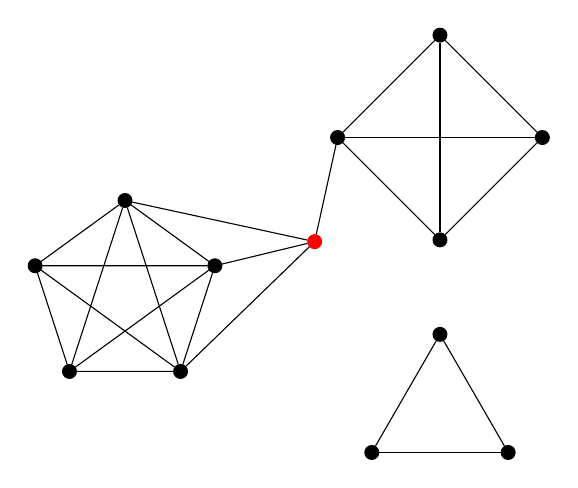
\begin{tikzpicture}[
    mycircle/.style={
        circle,
        draw=black,
        fill=black,
        fill opacity = 1,
        inner sep=0pt,
        minimum size=5pt,
        font=\small},
    nocircle/.style={
        circle,
        draw=black,
        fill=black,
        fill opacity = 1,
        inner sep=0pt,
        minimum size=0.45pt,
        font=\small},
    targetcircle/.style={
        circle,
        draw=red,
        fill=red,
        fill opacity = 1,
        inner sep=0pt,
        minimum size=5pt,
        font=\small},
    myarrow/.style={-},
    dottedarrow/.style={-,dashed},
    thiccarrow/.style={-,line width=0.9pt},
    node distance=1.2cm and 1.5cm
]
\begin{scope}
    \begin{scope}[rotate=-90]
        \foreach \x/\y in {0/a,90/b,180/c, 270/d}{ % color in outer layer
        \node[mycircle] (\y) at (canvas polar cs: radius=1.3cm,angle=\x){};
        }
    \end{scope}

    \path[every node/.style={font=\sffamily\small}]
        (a) edge [color=black] (b)
        (a) edge [color=black] (c)
        (a) edge [color=black] (d)
        (b) edge [color=black] (c)
        (b) edge [color=black] (d)
        (c) edge [color=black] (d);
\end{scope}

\begin{scope}[xshift=-4cm, yshift=-2cm, rotate=-72]
    \begin{scope}[rotate=90]
        \foreach \x/\y in {0/0,72/1,144/2, 216/3, 288/4}{ % color in outer layer
        \node[mycircle] (\y) at (canvas polar cs: radius=1.2cm,angle=\x){};
        }
    \end{scope}

    \path[every node/.style={font=\sffamily\small}]
        (0) edge [color=black] (1)
        (0) edge [color=black] (2)
        (0) edge [color=black] (3)
        (0) edge [color=black] (4)
        (1) edge [color=black] (2)
        (1) edge [color=black] (3)
        (1) edge [color=black] (4)
        (2) edge [color=black] (3)
        (2) edge [color=black] (4)
        (3) edge [color=black] (4);

    \node[targetcircle] (x) at (0.1, 2.5) {};

    \path[every node/.style={font=\sffamily\small}]
        (x) edge [color=black] (0)
        (x) edge [color=black] (1)
        (x) edge [color=black] (4)
        (x) edge [color=black] (d);
\end{scope}

\begin{scope}[yshift=-3.5cm, xshift=0cm]
    \begin{scope}[rotate=90]
        \foreach \x/\y in {0/0,120/1,240/2}{ % color in outer layer
        \node[mycircle] (\y) at (canvas polar cs: radius=1cm,angle=\x){};
        }
    \end{scope}

    \path[every node/.style={font=\sffamily\small}]
        (0) edge [color=black] (1)
        (0) edge [color=black] (2)
        (1) edge [color=black] (2);
\end{scope}
\end{tikzpicture}
\end{document}}
            \caption{$t=3$}
            \label{3community train series, c}
        \end{subfigure}
        \caption{First 3 time steps of the simplified, synthetic 3 community networks. The red node represents the target node which we aim to model. The 3, 4, and 5 node components represent the 30, 35, and 40 node communities respectively. At each time step the one edge is removed between the target node and the community it has the fewest connections with.}
        \label{3community train series}
    \end{figure}
     
    The three community was chosen as a best case scenario system to model. It has been constructed to avoid the challenges that are posed by the 2 community and long tail systems. That is, because in this system the target node is moving away from its least similar community, not moving from one community to another, it is not required to overcome the issue of symmetrical input. And because there are no long tails in this system, the SVD is able to capture a lot of the system with a low dimensional.

\end{section}

\begin{section}{Results and Discussion}
    \subsection{Embedding Prediction}
        For each of these systems, we took embedded the temporal network in two dimensions at each time step. The temporal embeddings were then divided into a training set of 20 and a testing set of 15. The output of the trained neural networks was then used to train a symbolic regression model that could use a simple set of addition, subtraction, division, and multiplication. 

        We predicted the evolution of the 2 community, long tail, and 3 community systems for 15 time steps after the training period using both a NNDE model and a symbolic regression model.

        To compare our models, we look at the distance of the predictions to the embedding of the target node. Note that this does not include the loss from the SVD, which con be reduced by increasing the number of singular values taken in for the SVD.
        
        To find the predicted probability of the edges of node $i$, $\mathbb{P}(i \leftrightarrow j:j\in V\smallsetminus \{i\})$, we use: 
        \begin{align}
            _tA_{i,\cdot} &\approxeq (\bar p) _t\hat R
        \end{align}
        Where $\bar p$ is the predicted location of the target node $i$ in the embedding at time $t$.

        To find calculate the loss of our prediction at time $t$, we use:
        \begin{align}
            \bar j &= V \smallsetminus \{i\}  \\
            L &= \frac{1}{||\bar j||}\sum{(_t\hat A_{i,\cdot} \hat R_{\cdot,\bar j} - (\bar p) _t\hat R_{\cdot,\bar j})^2}
        \end{align}
        That is the mean squared error between the probabilities given by the true embedding and the prediction.
        
        When we do this for the SVD, NN, and symbolic regression, we get \autoref{loss_table}.
        \begin{figure}
            \begin{center}
                \begin{tabular}{| m{0.17\textwidth} | m{0.25\textwidth} | m{0.25\textwidth} |}
                    \hline
                    Sequence & Neural Network Prediction Loss & Symbolic Regression Prediction Loss\\ 
                    \hline
                    \hline
                    2 Community & 5.784 & 10.16\\ 
                    \hline 
                    Long Tail  & 3.858 & 0.057 \\ 
                    \hline 
                    3 Community & 6.597 & 2.047 \\ 
                    \hline 
                \end{tabular}
                \end{center}
                \caption{A summary of the mean loss of the predictions at the fifth to ninth time steps. The neural network and symbolic prediction loss comes from the RDPG being reconstructed but with the position of the target node replaced with the location of the respective prediction. Loss is calculated as the mean squared error between the prediction predicted edge probability and the edge probability of the embedding.}
                \label{loss_table}
        \end{figure}

        As can be seen in \autoref{loss_table}, the symbolic regression model performed better for both the long tail system and the 3 community system. However, for the 2 community system the symbolic regression model performed notably worse. 

        The loss of one system should not be compared with another. That is the 2 community losses should not be compared to the long tail. This is because the long tail system will only ever have one edge to predict, whereas the 2 community will have 50 edges that need to be predicted.

        Instead, we may compare predictions within the same system. However, we do not see much difference between these predictions, and so we plot our predictions at each time step to further understand the behavior of our framework.

    \subsection{Further Exploration}
        In fig \autoref{2community series}, \autoref{longtail series},\autoref{3community series} the purple points are the embedded coordinates of the node in each of the communities. Each cluster is one separate community. The green point is the true coordinate of the embedded target node at each time step. The blue point is our neural network model prediction at each time step. The orange point is the symbolic regression prediction. 
        
        To illustrate how the changing structure of the network is represented in the embedding, we give a brief description of the movement of the target node throughout the 2 community system below.

        As the time progresses, we see the true node move from one community cluster to the other. This is because, at the beginning of the training phase, the target node starts as very similar to the first community (as it has many connections with nodes in that community) and as time progresses, it gradually becomes less and less similar to the first community and more similar to the second (as the edges between the target node and the first community are replaced with edges to the second community). Because the SVD embeds nodes with many of the same connections close to each other, we see the target node move towards the second community.

        \subsubsection{2 Community}
            \begin{figure}
                \foreach \i in {3,6,9,12,15} {%
                    \begin{subfigure}[p]{0.4\textwidth}
                        \includegraphics[width=\linewidth]{../Code/Plots/Test Only/2communities/2communities \i \space small net.png}
                        \caption{t=\i}
                        \label{2community series \i}
                    \end{subfigure}\quad
                }
                \caption{2 Community test series. This series shows the comparison of the neural network model, the symbolic regression model trained on the neural network model, and the true solution of the two community system.}
                \label{2community series}
            \end{figure}
            We see the neural network model quickly jumps to around $(-0.5,-0.5)$ where it sits for the entire simulation. This happened across many training periods; either a few time steps after the training period or right at the end of it, the neural network model moved towards a stable point where it remained for the test period.

            Similarly, the symbolic regression prediction remains close to the neural network prediction at the beginning of the test period, but towards the end of the test period begin to drift away. 
            
            The poor predictive behaviour of the models may be attributed to this being a symmetrical problem. That is, with the same set of distances as input into the model, the target node needs to move away from its nearest neighbours in the first half, then move towards its nearest neighbours in the second half. 
            
            Potential ways of breaking this symmetry may be to include information of the previous time step, or to include the absolute position of the target node as input into the neural network.

        \subsubsection{Long Tail}
            \begin{figure} 
                \foreach \i in {3,6,9,12,15} {%
                    \begin{subfigure}[p]{0.4\textwidth}
                        \includegraphics[width=\linewidth]{../Code/Plots/Test Only/longTail/longTail \i \space small net.png}
                        \caption{t=\i}
                        \label{longtail series \i}
                    \end{subfigure}\quad
                }
                \caption{Long Tail test series. This series shows the comparison of the neural network model, the symbolic regression model trained on the neural network model, and the true solution of the long tail system.}
                \label{longtail series}
            \end{figure}
            In fig \autoref{longtail series} we see the true embedding of the target node jump from one arm to the other at each time step. It is clear that neither the symbolic regression model nor the neural network model capture this movement. 
            
            However, the symbolic regression model maintains an appropriate distance from the origin oven if it does not follow the movement of the target node.

            We see that neither the neural network model capture the movement of the target node to any real extent. One reason for this may be that by the time the system progresses to the test section the number of nearest neighbours (k=15) means that the input for the model no longer includes the large community used to orient the system. Because of this, the model will essentially be given the same input at every time step, but will have to somehow produce the alternating behaviour of the target node. This again is an issue of symmetry. 
            
            The solutions to symmetry in this problem would be the same as for the two community system. That is, to break the symmetry by including the absolute position of the target node as input for the model, or to have multiple time steps as input. 
            
            Another potential solution we might consider in this instance, could be increasing the number of nearest neighbours so that the model always has a reference point. That is, the model would have the position of the large community as input. This solution would not generalise well however, as, in general, we may not know how long a tail could be, and therefore how many nearest neighbours to include.


        \subsubsection{Three Community}
            \begin{figure}
                \foreach \i in {3,6,9,12,15} {%
                    \begin{subfigure}[p]{0.4\textwidth}
                        \includegraphics[width=\linewidth]{../Code/Plots/Test Only/3community/3community \i \space small net.png}
                        \caption{t=\i}
                        \label{3community series \i}
                    \end{subfigure}\quad
                }
                \caption{3 community test series. This series shows the comparison of the neural network model, the symbolic regression model trained on the neural network model, and the true solution of the 3 community system.}
                \label{3community series}
            \end{figure}
            In fig \autoref{3community series} we see both models move roughly in the same direction as the target node. The neural network however moves quickly ahead of the target node and, as it does, away from the precise direction of the target node. 
            
            In contrast, the symbolic regression model maintains a very small distance to the target node.

            This system was constructed to avoid the symmetrical input of the other two systems. The models built for the 3 community system are by far the most accurate, with the symbolic regression model being particularly impressive. 
            
            This supports the notion that symbolic regression, when the training data is non-symmetrical, can give more robust predictive models than a NNDE alone.

            
            \subsection{Summary}
                We see a large difference in the training predictions between the 2 and 3 community systems. In the 2 community system, even in the training period, the predictions tended to wander and be less accurate. Whereas the 3 community training predictions remained very close to the true target node. The movement of the target node in the embedding was very similar between the two systems, and so the difference seems to be that the 2 community has symmetrical inputs.

                These were trained on a relatively small neural network (4 hidden layers (64,8,8,8)).


\end{section}

\begin{section}{Code}
    \subsection{Summary}
    The idea of this code is to provide a foundation for a streamline research into temporal network modelling. To that end it is planned to be compatible with popular Julia packages such as Graphs, the SciML ecosystem, and EcologicalNetworks.
    \subsection{Statement of Need}
    

    \subsection{Package Methods}

    \subsection{Comparable Methods and Related Work}
    Teneto Python

    packages("sna")  R
    packages("tsna")
    packages("ndtv")

    EvolvingGraphs Julia

    \subsection{Past and Ongoing Research}
    Wrote code that is general
    
    Made a structure (TemporalNetworkEmbedding)

    Useful functions include nearestNeighbours, and constructRDPG.
\end{section}
% \begin{section}{Conclusion}
%     In this paper, we proposed a novel framework for modelling temporal networks. We then tested this framework on three types of small, synthetic network sequences. Throughout these tests the neural network performed generally more poorly than the symbolic regression model, with the large three community sequence being especially notable due to th symbolic regression remaining so close to the target node throughout the test period. 
% \end{section} 


\printbibliography

\end{document} 

% draft for miguel
% all absolute pos of nodes
% polar positions

% questions for Giulio:
%     Why both NN and sym reg not just sym reg
%     Why cos dist 